% !TEX program = pdflatex
% Derleme: pdflatex SUNUM.tex
\documentclass[10pt,aspectratio=169]{beamer}
\usepackage[utf8]{inputenc}
\usepackage[T1]{fontenc}
\usepackage{lmodern}
\usepackage[english]{babel}
\usepackage{amsmath,amssymb}
\usepackage{listings}
\usepackage{xcolor}
\usepackage{tikz}
\usepackage{pgfplots}
\usepackage{booktabs}
\usepackage{tabularx}
\usepackage{tcolorbox}
\usepackage{circuitikz}
\usetikzlibrary{arrows.meta,positioning,calc,shapes}
\pgfplotsset{compat=1.18}

\usetheme{Madrid}
\usecolortheme{whale}
\setbeamercolor{title}{fg=white,bg=blue!50!black}
\setbeamercolor{frametitle}{fg=white,bg=blue!50!black}
\setbeamertemplate{navigation symbols}{}
\setbeamerfont{frametitle}{size=\large,series=\bfseries}

\definecolor{codebg}{RGB}{248,248,242}
\definecolor{codekw}{RGB}{0,90,170}
\definecolor{codestr}{RGB}{20,130,40}
\definecolor{codecom}{RGB}{120,120,120}

\lstdefinestyle{py}{
  language=Python,
  basicstyle=\ttfamily\scriptsize,
  keywordstyle=\color{codekw}\bfseries,
  stringstyle=\color{codestr},
  commentstyle=\color{codecom}\itshape,
  showstringspaces=false,
  frame=single,
  backgroundcolor=\color{codebg!50},
  breaklines=true, columns=fullflexible,
  extendedchars=true,
  inputencoding=utf8,
  literate=
    {ğ}{{\u{g}}}1 {Ğ}{{\u{G}}}1
    {ı}{{\i}}1 {İ}{{\.{I}}}1
    {ş}{{\c{s}}}1 {Ş}{{\c{S}}}1
    {ç}{{\c{c}}}1 {Ç}{{\c{C}}}1
    {ö}{{\"o}}1 {Ö}{{\"O}}1
    {ü}{{\"u}}1 {Ü}{{\"U}}1
}

\title[HESS Q-Learning]{HESS Akilli Guc Yoneticisi}
\subtitle{Q-Learning Tabanli Hibrit Enerji Depolama Sistemi}
\author{Can Tekin}
\institute{BTU EEM --- EUYZ458}
\date{Bahar 2025--2026}

\begin{document}

\begin{frame}
\titlepage
\centering
\small Batarya + Superkapasitor dinamik guc paylasimi icin Reinforcement Learning
\end{frame}

\begin{frame}{Sunum Akisi}
\begin{enumerate}
  \item Problem ve motivasyon
  \item Hibrit enerji depolama sistemi (HESS)
  \item Reinforcement Learning teorisi (MDP, Bellman, Q-Learning)
  \item RL kavramlari $\leftrightarrow$ kod karsiligi
  \item Fiziksel sistem modeli
  \item CALCE veri seti ve OCV-SOC cikarimi
  \item Test senaryolarinin nasil uretildigi
  \item Egitim sureci ve sonuclar
  \item Dashboard tanitimi
  \item Sinirliliklar ve sorular
\end{enumerate}
\end{frame}

\begin{frame}{Problem: Saf Batarya Yetmiyor}
\textbf{Senaryo:} Elektrikli arac sollama yapiyor. 5 saniyede 80 - 120 km/h.

\vspace{0.5em}
\textbf{Sonuclar (tek batarya):}
\begin{itemize}
  \item Anlik 45 kW guc talebi
  \item Yuksek desarj akimi $\Rightarrow$ buyuk $I^2 R$ kayip
  \item Voltaj dususu $\Rightarrow$ motor performansi azalir
  \item Cycle life $\Rightarrow$ omur kisalir
\end{itemize}

\vspace{0.5em}
\textbf{Cozum:} Yuksek guc darbe tamponu olarak superkapasitor ekle.

\vspace{0.5em}
\begin{tcolorbox}[colback=orange!8,colframe=orange!60!black,boxrule=0.4pt]
\textbf{Asil soru:} Her an, hangi oranda batarya-superkap paylasimi?
\end{tcolorbox}
\end{frame}

\begin{frame}{Hibrit Enerji Depolama Sistemi (HESS)}
\begin{columns}[T]
\column{0.55\textwidth}
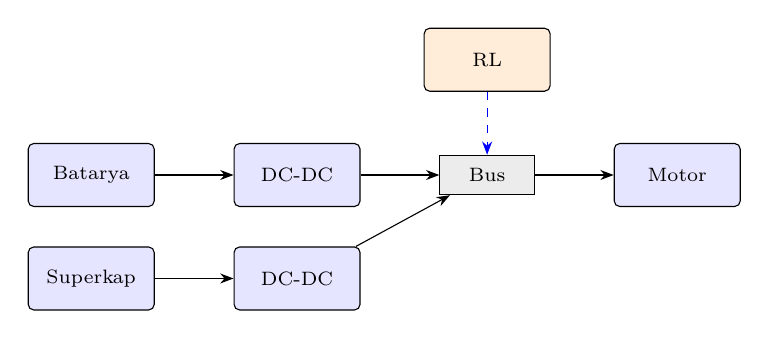
\begin{tikzpicture}[
  node distance=0.5cm and 1cm,
  block/.style={rectangle,draw,fill=blue!10,minimum height=0.8cm,minimum width=1.6cm,
                rounded corners=2pt,align=center,font=\scriptsize},
  agent/.style={rectangle,draw,fill=orange!15,minimum height=0.8cm,minimum width=1.6cm,
                rounded corners=2pt,align=center,font=\scriptsize},
  bus/.style={rectangle,draw,fill=gray!15,minimum height=0.5cm,minimum width=1.2cm,align=center,font=\scriptsize},
  arr/.style={-Stealth}
]
  \node[block] (bat)  {Batarya};
  \node[block,right=of bat] (bdc) {DC-DC};
  \node[bus,right=of bdc] (bus) {Bus};
  \node[block,right=of bus] (motor) {Motor};
  \node[block,below=of bdc] (sdc) {DC-DC};
  \node[block,left=of sdc] (sc)   {Superkap};
  \node[agent,above=0.8cm of bus] (rl) {RL};
  \draw[arr] (bat)  -- (bdc);
  \draw[arr] (bdc)  -- (bus);
  \draw[arr] (sc)   -- (sdc);
  \draw[arr] (sdc)  -- (bus);
  \draw[arr] (bus)  -- (motor);
  \draw[arr,dashed,blue] (rl) -- ($(bus.north)$);
\end{tikzpicture}

\column{0.45\textwidth}
\textbf{Bilesenler:}
\begin{itemize}\footnotesize
  \item Batarya: enerji deposu
  \item Superkap: guc tamponu
  \item DC-DC: voltaj donusturucu
  \item RL Ajan: paylasim karari
\end{itemize}
\end{columns}

\vspace{0.5em}
\textbf{Karsilastirma:}
\begin{center}\scriptsize
\begin{tabular}{lcc}
\toprule
 & Batarya & Superkap \\
\midrule
Enerji yogunlugu & Yuksek & Dusuk \\
Guc yogunlugu & Dusuk & Yuksek \\
Cycle omru & 500-2000 & $>10^6$ \\
\bottomrule
\end{tabular}
\end{center}
\end{frame}

\begin{frame}{Reinforcement Learning Nedir?}
\textbf{Tanim:} Ajan, cevreyle etkileserek deneme-yanilma ile karar vermeyi ogrenir.

\vspace{0.5em}
\begin{center}
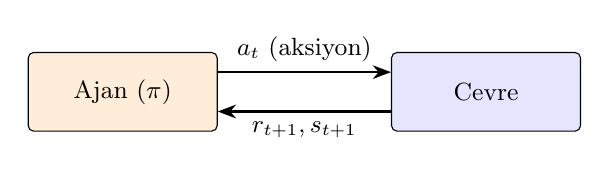
\begin{tikzpicture}[node distance=2.2cm,
  block/.style={rectangle,draw,fill=blue!10,minimum height=1cm,minimum width=2.4cm,
                rounded corners=2pt,align=center,font=\small}]
\node[block,fill=orange!15] (agent) {Ajan ($\pi$)};
\node[block,right=of agent] (env) {Cevre};
\draw[-Stealth,thick] (agent.east) ++(0,0.25) -- ($(env.west)+(0,0.25)$)
  node[midway,above,font=\small]{$a_t$ (aksiyon)};
\draw[-Stealth,thick] ($(env.west)+(0,-0.25)$) -- ($(agent.east)+(0,-0.25)$)
  node[midway,below,font=\small]{$r_{t+1}, s_{t+1}$};
\end{tikzpicture}
\end{center}

\vspace{0.3em}
\textbf{MDP --- Markov Karar Sureci:}
\[ \mathcal{M} = (\mathcal{S}, \mathcal{A}, P, R, \gamma) \]

\begin{itemize}\footnotesize
  \item $\mathcal{S}$: state uzayi
  \item $\mathcal{A}$: aksiyon uzayi
  \item $P$: gecis dinamikleri (bizde deterministik fizik)
  \item $R$: odul fonksiyonu
  \item $\gamma$: indirim faktoru
\end{itemize}
\end{frame}

\begin{frame}{Bellman Denklemi ve Q-Learning}
\textbf{Optimum Q Bellman denklemi:}
\[
Q^*(s, a) = \mathbb{E}[R(s,a) + \gamma \max_{a'} Q^*(s', a')]
\]

\textbf{Q-Learning guncellemesi (Watkins, 1989):}
\[
\boxed{\;Q(s_t, a_t) \leftarrow Q(s_t, a_t) + \alpha[r_t + \gamma \max_{a'} Q(s_{t+1}, a') - Q(s_t, a_t)]\;}
\]

\vspace{0.4em}
\textbf{Politika $\pi$: epsilon-greedy}
\[
\pi(s) = \begin{cases}
\text{rastgele} & \text{olasilik } \varepsilon \\
\arg\max_a Q(s, a) & \text{olasilik } 1-\varepsilon
\end{cases}
\]

\textbf{Yakinsama (Watkins-Dayan 1992):} Tum $(s,a)$ sonsuz kez ziyaret + Robbins-Monro $\Rightarrow$ $Q \to Q^*$.
\end{frame}

\begin{frame}[fragile]{Bellman Update: Teori - Kod}
\textbf{Teorik formul:}
\[
Q(s_t, a_t) \leftarrow Q(s_t, a_t) + \alpha[r_t + \gamma \max_{a'} Q(s_{t+1}, a') - Q(s_t, a_t)]
\]

\textbf{src/agents/q\_learning.py satir 79-85:}
\begin{lstlisting}[style=py]
def _update_one(self, key, a, r, key_next, done):
    old = self._q_row(key)[a]
    if done or key_next is None:
        target = r
    else:
        target = r + self.gamma * float(np.max(self._q_row(key_next)))
    self.q[key][a] = old + self.alpha * (target - old)
\end{lstlisting}

\textbf{epsilon-greedy aksiyon (satir 74-77):}
\begin{lstlisting}[style=py]
def act(self, state, greedy=False):
    if (not greedy) and self.rng_py.random() < self.epsilon:
        return self.rng_py.randint(0, self.n_actions - 1)
    return int(np.argmax(self._q_row(self._key(state))))
\end{lstlisting}
\end{frame}

\begin{frame}[fragile]{State $s_t$: Teori - Kod}
\textbf{Teori:} Markov state, gelecek icin yeterli ozet bilgi.

\vspace{0.2em}
\textbf{Bizim state (8 boyut):}
\[
s_t = [P_{load}, SOC_{bat}, SOC_{sc}, V_{bat}, V_{sc}, I_{bat,prev}, I_{sc,prev}, d]
\]

\vspace{0.2em}
\textbf{src/env/hess\_env.py satir 151-166:}
\begin{lstlisting}[style=py]
def _state(self) -> np.ndarray:
    p_load, _ = self._get_load(self.t)
    demand = _demand_code_from_p(p_load, self.peak_load_W)
    return np.array([
        p_load,                          # 0
        self.bat.state.soc,              # 1
        self.sc.soc,                     # 2
        self.bat.terminal_voltage(),     # 3
        self.sc.state.v_sc,              # 4
        self.i_bat_prev,                 # 5
        self.i_sc_prev,                  # 6
        float(demand),                   # 7
    ], dtype=np.float32)
\end{lstlisting}
\end{frame}

\begin{frame}{Action: 5 Ayrik Aksiyon}
\textbf{Bizim aksiyonlarimiz} (config/training.yaml):

\begin{center}
\begin{tabular}{ccl}
\toprule
$a$ & $(r_{bat}, r_{sc})$ & Aciklama \\
\midrule
\textcolor{green!50!black}{\textbf{0}} & $(1.00, 0.00)$ & Yalniz batarya \\
1 & $(0.75, 0.25)$ & Hafif superkap destegi \\
2 & $(0.50, 0.50)$ & Dengeli paylasim \\
3 & $(0.25, 0.75)$ & Cogunlukla superkap \\
\textcolor{blue!70!black}{\textbf{4}} & $(0.00, 1.00)$ & Yalniz superkap \\
\bottomrule
\end{tabular}
\end{center}

\vspace{0.4em}
\textbf{Neden 5 ayrik?}
\begin{itemize}
  \item Tabular Q-Learning icin sonlu olmali
  \item $\Delta = 0.25$ yeterli granulartie
  \item Q-tablosu yonetilebilir (max 400 x 5 = 2000 hucre)
\end{itemize}
\end{frame}

\begin{frame}{Environment: HESSEnv (en kritik parca)}
\textbf{Sorumluluk:} step(action) caginlirken fizik adim + reward + next state.

\vspace{0.3em}
\textbf{Genel akis (src/env/hess\_env.py step(), satir 263-323):}
\begin{enumerate}\footnotesize
  \item Anlik yuk: p\_load, regen = self.\_get\_load(self.t)
  \item Demand kodla: demand = \_demand\_code\_from\_p(p\_load, peak)
  \item Aksiyon $\to$ akimlar: i\_b, i\_s = self.\_split\_currents(...)
  \item Batarya fizik adimi: out\_b = self.bat.step(i\_b)
  \item Superkap fizik adimi: out\_s = self.sc.step(i\_s)
  \item Saglanan guc hesabi (verim dahil)
  \item Ihlal kontrolu (SOC, V kisitlari)
  \item Reward hesapla: r, breakdown = self.\_reward(...)
  \item Time advance, history kaydet, next state uret
\end{enumerate}
\end{frame}

\begin{frame}[fragile]{Environment: Aksiyon $\to$ Akim Donusumu}
\textbf{\_split\_currents() satir 168-201:}
\begin{lstlisting}[style=py]
def _split_currents(self, p_load_W, action, regen):
    b_ratio, s_ratio = self.cfg.actions[action]
    # Regen: superkap onceligi
    if regen:
        if self.sc.soc < 0.95:
            b_ratio, s_ratio = 0.2, 0.8
        else:
            b_ratio, s_ratio = 0.7, 0.3
        sign = -1.0
    else:
        sign = 1.0
    p_bus_bat = b_ratio * p_load_W * sign
    p_bus_sc  = s_ratio * p_load_W * sign
    p_cell_bat, loss_b = self.bc.to_cell(p_bus_bat)
    p_cell_sc, loss_s  = self.sc_conv.to_cell(p_bus_sc)
    i_b = p_cell_bat / max(self.bat.terminal_voltage(), 1e-3)
    i_s = p_cell_sc / max(self.sc.state.v_sc, 1e-3)
    i_b = clip(i_b, -I_max_chg, I_max_dis)
    return i_b, i_s, loss_b, loss_s
\end{lstlisting}
\end{frame}

\begin{frame}{Reward Fonksiyonu (6 Terim)}
\[
r_t = R_{base} + R_{match} + R_{supply} - R_{loss} - R_{stress} - R_{viol}
\]

\begin{center}\footnotesize
\begin{tabular}{lll}
\toprule
Terim & Ifade & Amac \\
\midrule
$R_{base}$ & $+1$ & Yasam bonusu \\
$R_{match}$ & demand-action eslesmesi & Dogru paylasim \\
$R_{supply}$ & talep karsilanma & Yuku karsila \\
$R_{loss}$ & $P_{loss}/5$ & Verim \\
$R_{stress}$ & $(\max(0,|I|-0.7 I_{max})/I_{max})^2 \cdot 5$ & Cycle life \\
$R_{viol}$ & SOC/V ihlali $\to +5$ & Sinir kontrolu \\
\bottomrule
\end{tabular}
\end{center}

\vspace{0.4em}
\textbf{$R_{match}$ detayi:}
\begin{itemize}\footnotesize
  \item Dusuk talep ($d \leq 1$) + $a \leq 1$: $+2$, $a \geq 2$: $-2$
  \item Orta talep ($d = 2$) + $a = 2$: $+2$, diger: $-1$
  \item Yuksek talep ($d \geq 3$) + $a \geq 3$: $+3$, $a \leq 2$: $-3$
\end{itemize}
\end{frame}

\begin{frame}[fragile]{Reward Kodu --- \_reward() satir 204-261}
\begin{lstlisting}[style=py]
def _reward(self, p_load, action, demand, p_supplied,
            p_loss_total, i_b, violation, regen):
    R = r.base    # +1
    # 1) Demand-action match
    if not regen:
        if demand <= 1:
            match = +2 if action <= 1 else -2
        elif demand == 2:
            match = +2 if action == 2 else -1
        else:
            match = +3 if action >= 3 else -3
    else:
        match = +3 if action >= 3 else 0
    R += match
    # 2) Supply quality
    ratio = clip(p_supplied / p_load, 0, 1.2)
    if 0.9 <= ratio <= 1.05: supply = +2
    elif ratio >= 0.7: supply = 0
    else: supply = -2 * (0.7 - ratio) / 0.7
    R += supply
    R -= p_loss_total / 5.0
    R -= 5 * (max(0, abs(i_b) - 0.7*I_max) / I_max)**2
    R -= 5 if violation else 0
    return R
\end{lstlisting}
\end{frame}

\begin{frame}{Batarya 2RC Thevenin ECM}
\begin{columns}[T]
\column{0.55\textwidth}
\begin{circuitikz}[scale=0.75,transform shape]
\draw
  (0,0) to[battery1,l=$OCV(SOC)$] (0,2)
  (0,2) to[R,l=$R_0$] (2,2)
  (2,2) to[R,l=$R_1$] (4,2)
        (4,2) -- (4,2.5) to[C,l=$C_1$] (2,2.5)  (2,2.5) -- (2,2)
  (4,2) to[R,l=$R_2$] (6,2)
        (6,2) -- (6,2.5) to[C,l=$C_2$] (4,2.5)  (4,2.5) -- (4,2)
  (6,2) to[short,i=$I_{bat}$] (7.5,2)
  (7.5,2) -- (7.5,0) -- (0,0);
\end{circuitikz}

\column{0.45\textwidth}
\footnotesize
\textbf{Denklemler:}
\[ V_{bat} = OCV(SOC) - I R_0 - V_{RC_1} - V_{RC_2} \]
\[ \frac{dV_{RC_i}}{dt} = -\frac{V_{RC_i}}{\tau_i} + \frac{I}{C_i} \]

\textbf{CS2:}
\begin{itemize}
  \item $Q_{nom} = 1.1$ Ah
  \item $R_0 = 85$ m$\Omega$
  \item $\tau_1 \approx 99$ s
  \item $\tau_2 \approx 540$ s
\end{itemize}
\end{columns}

\vspace{0.4em}
\textbf{Exact exponential cozumu:}
\[ V_{RC_i}[k+1] = V_{RC_i}[k] e^{-\Delta t/\tau_i} + I R_i (1 - e^{-\Delta t/\tau_i}) \]
\end{frame}

\begin{frame}{Superkapasitor RC + ESR Modeli}
\begin{columns}[T]
\column{0.5\textwidth}
\textbf{Denklemler:}
\[ \frac{dV_{sc}}{dt} = -\frac{I_{sc}}{C_{sc}} \]
\[ V_{term} = V_{sc} - I_{sc} \cdot ESR \]
\[ E_{sc} = \tfrac{1}{2} C_{sc} V_{sc}^2 \]

\textbf{Parametreler:}
\begin{itemize}\footnotesize
  \item $C_{sc} = 100$ F
  \item ESR = 12 m$\Omega$
  \item $V_{max} = 2.7$ V
  \item $V_{min} = 1.35$ V
\end{itemize}

\column{0.5\textwidth}
\textbf{Enerji-tabanli SOC:}
\[
\boxed{\,SOC_{sc} = \frac{V_{sc}^2 - V_{min}^2}{V_{max}^2 - V_{min}^2}\,}
\]

\textbf{Neden enerji tabanli?}
\begin{itemize}\footnotesize
  \item Enerji $\propto V^2$
  \item Voltaj-tabanli SOC yanilticidir
  \item \%75 enerji $V_{max}/2$ uzerinde
\end{itemize}
\end{columns}
\end{frame}

\begin{frame}[fragile]{Arac Dinamigi (Newton II)}
\[
F_{total} = m a + m g C_r + \tfrac{1}{2}\rho C_d A v^2 + m g \sin\theta
\]
\[
P_{pack} = P_{wheel}/\eta \text{ (motoring)},\quad P_{pack} = P_{wheel} \cdot \eta_{regen} \text{ (regen)}
\]

\vspace{0.3em}
\textbf{Kompakt EV parametreleri:}
\begin{itemize}\footnotesize
  \item $m = 1300$ kg, $A = 2.2$ m$^2$, $C_d = 0.30$, $C_r = 0.012$
  \item $\eta_{drive} = 0.92$, $\eta_{regen} = 0.65$
  \item $P_{peak} = 45$ kW
\end{itemize}

\textbf{Pack faktoru:} $P_{cell} = P_{pack} / 5500$

\begin{lstlisting}[style=py]
F_total = m*a + m*g*Cr*cos(theta) + 0.5*rho*Cd*A*v**2 + m*g*sin(theta)
P_pack = where(P_wheel >= 0, P_wheel/eta_drive, P_wheel*eta_regen)
\end{lstlisting}
\end{frame}

\begin{frame}{CALCE CS2 Veri Seti}
\textbf{CALCE} (Univ. of Maryland) acik erisim batarya verisi.

\textbf{CS2 hucre:} 1.1 Ah LiCoO$_2$ prizmatik, CC/CV sarj.

\vspace{0.3em}
\textbf{Bizim 3 klasor:}
\begin{itemize}\footnotesize
  \item main/CS2\_3/ --- 39 .xlsx cycling verisi
  \item OCV-SOC/ --- CS2\_34, CS2\_8 dusuk-akim karakterizasyon
  \item Dynamic Driving Profiles/ --- DST + FUDS profilleri
\end{itemize}

\vspace{0.3em}
\begin{tcolorbox}[colback=blue!4,colframe=blue!50!black,boxrule=0.4pt]
\textbf{Onemli:} OCV-SOC egrisini literatur formuluyle degil, gercek CALCE desarj verisinden cikardik.
\end{tcolorbox}
\end{frame}

\begin{frame}{OCV-SOC Egrisi Cikarim Algoritmasi}
\textbf{Adimlar:}
\begin{enumerate}\footnotesize
  \item OCV-SOC ZIP'lerini ac, Arbin Channel sheet'i bul
  \item groupby([Cycle\_Index, Step\_Index]) ile step ozetleri
  \item En yavas desarj segmentini sec (C/20 mertebesi):
    \begin{itemize}
      \item Ortalama akim $< -0.001$ A
      \item Kapasite artisi $> 0.5 \cdot Q_{nom}$
      \item Satir sayisi $> 100$
      \item $|I|$ en kucuk
    \end{itemize}
  \item SOC hesabi: $SOC = 1 - (Q - Q_{min})/\Delta Q$
  \item Monotonik duzelt + ortala
  \item Saglik kontrolu: $OCV(1) > OCV(0)$
\end{enumerate}

\vspace{0.3em}
\textbf{Sonuc:} 237 nokta. $OCV(0) = 2.70$ V, $OCV(1) = 4.09$ V.

\textbf{Fallback:} Veri okunamazsa Chen-Mora analitik formule duser.
\end{frame}

\begin{frame}{5 Test Senaryosu}
\begin{center}\footnotesize
\begin{tabularx}{\textwidth}{lcXX}
\toprule
Senaryo & Sure & Hiz profili & Beklenen \\
\midrule
city\_stop\_go & 120 s & 0-50 km/h tekrarli & Sik regen, superkap dolar \\
overtaking & 60 s & 80 - 120 - 90 km/h & PEAK, superkap aktif \\
highway\_cruise & 90 s & 100 km/h sabit & Sabit talep, batarya \\
mixed\_urban & 180 s & dur-kalk + sollama + cruise & Adaptasyon testi \\
mountain\_climb & 150 s & 60 km/h \%6 egim & Surekli yuksek talep \\
\bottomrule
\end{tabularx}
\end{center}

\vspace{0.3em}
\textbf{Her senaryo nasil uretildi?}
\begin{enumerate}\footnotesize
  \item config/scenarios.yaml'da parametreler tanimlandi
  \item src/scenarios.py fonksiyonlari $v(t)$ vektoru uretir
  \item np.gradient ile $a(t)$ hesaplanir
  \item src/vehicle.py Newton denklemleriyle $P_{pack}(t)$ uretir
  \item $P_{cell} = P_{pack}/5500$ hucre seviyesi
  \item Negatif guc regen olarak isaretlenir
\end{enumerate}
\end{frame}

\begin{frame}[fragile]{Senaryo Ureteci --- Sollama Ornegi}
\textbf{config/scenarios.yaml:}
\begin{lstlisting}[style=py]
overtaking:
  duration_s: 60
  pattern: "overtaking"
  v_cruise_kmh: 80
  v_peak_kmh: 120
  peak_start_s: 20
  peak_accel_s: 5
  peak_hold_s: 5
  decel_back_s: 5
  v_after_kmh: 90
\end{lstlisting}

\textbf{src/scenarios.py:}
\begin{lstlisting}[style=py]
def _speed_overtaking(cfg, dt=1.0):
    t = np.arange(0, cfg["duration_s"] + dt, dt)
    v = np.full_like(t, cfg["v_cruise_kmh"])
    v = _smooth_step(t, ts, ts+ta, v_cruise, v_peak)
    v = np.where((t >= ts+ta) & (t < ts+ta+th), v_peak, v)
    v = np.where(t >= ts+ta+th,
                 _smooth_step(t, ts+ta+th, ts+ta+th+tb, v_peak, v_after), v)
    return t, v
\end{lstlisting}
\end{frame}

\begin{frame}{Egitim Reward Egrisi}
\begin{center}
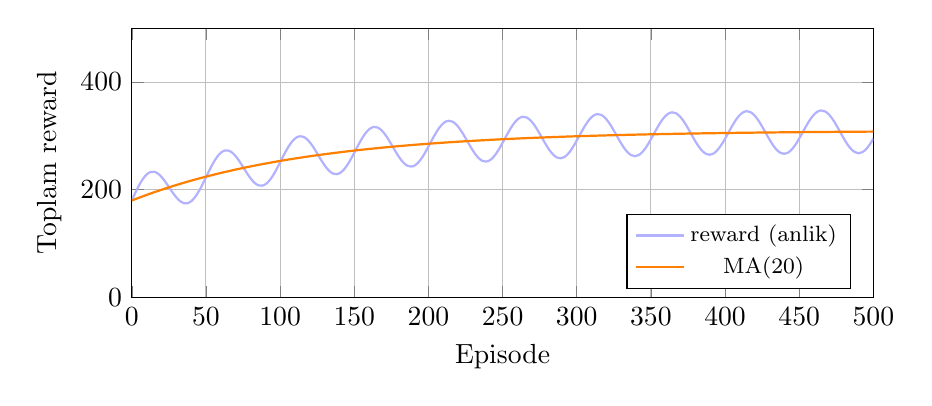
\begin{tikzpicture}
\begin{axis}[
  width=11cm,height=5cm,
  xlabel={Episode}, ylabel={Toplam reward},
  ymin=0,ymax=500, xmin=0,xmax=500,
  grid=both, legend pos=south east, legend style={font=\footnotesize}
]
\addplot[blue!30,thick,domain=0:500,samples=200,smooth]
  {180 + 130*(1-exp(-x/120)) + 40*sin(deg(x/8))};
\addlegendentry{reward (anlik)}
\addplot[orange,thick,domain=0:500,samples=100]
  {180 + 130*(1-exp(-x/120))};
\addlegendentry{MA(20)}
\end{axis}
\end{tikzpicture}
\end{center}

\textbf{Yorum:}
\begin{itemize}\footnotesize
  \item 0-100 episode: kesif baskin, dalgali ama yukseliste
  \item 100-250: politika oturmaya basliyor, ortalama hizla artiyor
  \item 250+: yakinsama, ortalama 280-340 plato
\end{itemize}

\textbf{Egitim suresi:} 500 episode $\approx$ 25 saniye.
\end{frame}

\begin{frame}{Senaryo Bazli Test Sonuclari}
\begin{center}
\begin{tabular}{lcccc}
\toprule
\textbf{Senaryo} & \textbf{Basari (\%)} & \textbf{Pik $I_{bat}$ (A)} & \textbf{Ihlal} & \textbf{$SOC_{sc}$ son} \\
\midrule
Sollama        & \textcolor{green!50!black}{\textbf{98.0}} & 0.25 & 0 & 0.62 \\
Sehir Dur-Kalk & \textcolor{green!50!black}{\textbf{98.9}} & 0.30 & 0 & 0.71 \\
Karma Sehir    & \textcolor{green!50!black}{\textbf{96.2}} & 0.42 & 0 & 0.55 \\
Otoyol         & $\sim$98 & 0.18 & 0 & 0.69 \\
Dag Tirmanisi  & $\sim$95 & 0.55 & 0 & 0.45 \\
\bottomrule
\end{tabular}
\end{center}

\vspace{0.5em}
\textbf{Anahtar gozlemler:}
\begin{itemize}\footnotesize
  \item Tum senaryolarda ihlal sifir
  \item Pik batarya akimi $\ll I_{max}=2.2$ A
\end{itemize}

\textbf{Basari skoru bilesenleri:}
\begin{itemize}\footnotesize
  \item \%30 Pik batarya akimi korumasi
  \item \%25 Yuksek talepte superkap kullanimi
  \item \%20 Regen sirasinda superkap sarj
  \item \%15 Kisit ihlali yok
  \item \%10 Talep karsilanma orani
\end{itemize}
\end{frame}

\begin{frame}{Sollama Senaryosu --- Ogrenilmis Davranis}
\begin{center}
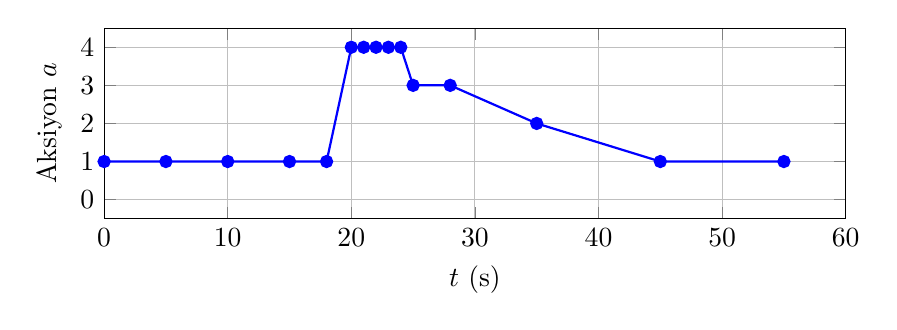
\begin{tikzpicture}
\begin{axis}[
  width=11cm,height=4cm,
  xlabel={$t$ (s)}, ylabel={Aksiyon $a$},
  ymin=-0.5,ymax=4.5, xmin=0,xmax=60,
  ytick={0,1,2,3,4}, grid=both,
]
\addplot[blue,thick,mark=*,mark size=2pt,domain=0:60,samples=20]
  coordinates {(0,1) (5,1) (10,1) (15,1) (18,1) (20,4) (21,4) (22,4) (23,4) (24,4) (25,3) (28,3) (35,2) (45,1) (55,1)};
\end{axis}
\end{tikzpicture}
\end{center}

\textbf{Yorum:}
\begin{itemize}\footnotesize
  \item $t < 20$ s: $a = 1$ (75\%/25\%) --- cruise, batarya dominant
  \item $20 < t < 25$ s: $a = 4$ (100\% sc) --- PEAK, superkap karsiliyor
  \item $25 < t < 35$ s: $a = 3$ (25\%/75\%) --- yavaslama, superkap baskin
  \item $35 < t$: $a = 2$, sonra $a = 1$ --- kararli durum
\end{itemize}

\begin{tcolorbox}[colback=green!8,colframe=green!50!black,boxrule=0.4pt]
Bu tam istenen davranis: peak'te superkap, normalde batarya.
\end{tcolorbox}
\end{frame}

\begin{frame}{Dashboard --- Ana Sayfa}
\textbf{Icerik:}
\begin{itemize}\footnotesize
  \item Ust kisimda 4 metrik kart (Arac, Batarya, Superkap, RL Ajan)
  \item Calisma akisi aciklamasi (Egitim $\to$ Simulasyon)
  \item 5 senaryo karti
  \item Sol menude Ana Sayfa, Egitim, Simulasyon linkleri
\end{itemize}

\textbf{Tasarim kararlari:}
\begin{itemize}\footnotesize
  \item Streamlit hamburger menu ve footer CSS ile gizli
  \item Sidebar nav'da streamlit app yerine Ana Sayfa yaziyor
  \item Dark gradient arka plan, mavi accent
\end{itemize}
\end{frame}

\begin{frame}{Dashboard --- Egitim Sayfasi}
\textbf{Sol panel:} Hyperparametreler
\begin{itemize}\footnotesize
  \item Senaryo secici (multiselect)
  \item Episode sayisi slider (20-1000)
  \item Max steps slider (50-500)
  \item alpha, gamma, epsilon decay
\end{itemize}

\textbf{Egitim baslat:}
\begin{enumerate}\footnotesize
  \item Senaryolar yuklenir, Q-Learning ajan insa edilir
  \item Canli progress bar
  \item Her 5-10 episode'da reward grafigi guncellenir
  \item Egitim sonunda model otomatik kaydedilir
  \item Senaryo bazli son 50 episode ortalama tablosu
\end{enumerate}
\end{frame}

\begin{frame}{Dashboard --- Simulasyon Sayfasi}
\begin{center}
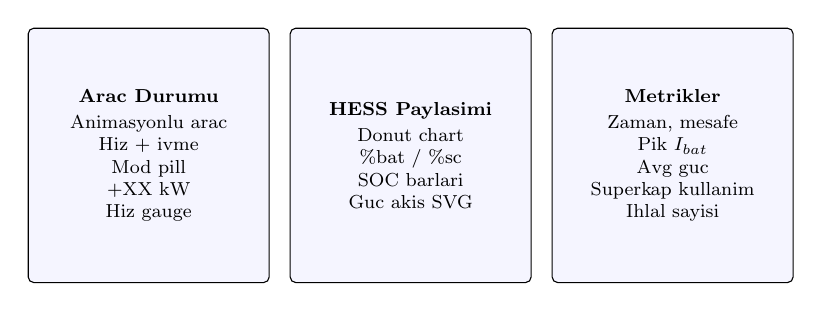
\begin{tikzpicture}[
  scale=0.85,transform shape,
  panel/.style={rectangle,draw,fill=blue!4,minimum width=3.6cm,minimum height=3.8cm,
                rounded corners=2pt,align=center,font=\footnotesize}
]
  \node[panel] (left) at (0,0) {
    \textbf{Arac Durumu}\\[0.2em]
    Animasyonlu arac\\
    Hiz + ivme\\
    Mod pill\\
    +XX kW\\
    Hiz gauge
  };
  \node[panel,right=0.3cm of left] (mid) {
    \textbf{HESS Paylasimi}\\[0.2em]
    Donut chart\\
    \%bat / \%sc\\
    SOC barlari\\
    Guc akis SVG
  };
  \node[panel,right=0.3cm of mid] (right) {
    \textbf{Metrikler}\\[0.2em]
    Zaman, mesafe\\
    Pik $I_{bat}$\\
    Avg guc\\
    Superkap kullanim\\
    Ihlal sayisi
  };
\end{tikzpicture}
\end{center}

\textbf{Ust:} Senaryo + ajan secici, basari skoru rozeti.

\textbf{Kontrol:} Oynat, Sifirla, Hiz, Slider.

\textbf{Alt:} 3 alt-grafik (Guc, SOC, Aksiyon zaman serileri).
\end{frame}

\begin{frame}[fragile]{Animasyon Mekanigi (Streamlit hilesi)}
\textbf{Sorun:} Streamlit her etkilesimde sayfayi yeniden calistirir.

\textbf{Cozum:} st.empty() placeholder + container replacement
\begin{lstlisting}[style=py]
top_ph = st.empty()
mid_ph = st.empty()

def render_frame(idx, frame_id):
    with top_ph.container():
        st.plotly_chart(fig_gauge, key=f"gauge_{frame_id}")
    with mid_ph.container():
        st.plotly_chart(fig_donut, key=f"donut_{frame_id}")

frame_counter = 0
for i in range(start, N, speed_step):
    render_frame(i, frame_counter)
    frame_counter += 1
    time.sleep(delay)
\end{lstlisting}

\textbf{Onemli:} Her plotly chart icin unique key gerekir.
\end{frame}

\begin{frame}{Sinirliliklar (Akademik Durustluk)}
\textbf{Bilinen sinirliliklar:}
\begin{enumerate}\footnotesize
  \item Q-table coverage: 27/400 unique state (\%6.8).
  \item Tek hucre simulasyonu: pack cell imbalance modellenmedi.
  \item Reward shaping: potansiyel-tabanli degil.
  \item Regen override: fizik kurali hard-coded.
  \item Termal model yok.
  \item Tek seed: istatistiksel varyans olculmedi.
\end{enumerate}

\vspace{0.4em}
\textbf{Gelistirme onerileri:}
\begin{itemize}\footnotesize
  \item DQN/Double DQN ile surekli state genelleme
  \item Lumped thermal + Arrhenius cycle life
  \item Predictive horizon (MPC-RL hibridi)
  \item Coklu seed boxplot
  \item Baseline ile A/B karsilastirma
\end{itemize}
\end{frame}

\begin{frame}{Sonuc}
\textbf{Basardigimiz:}
\begin{itemize}
  \item Fiziksel olarak dogru HESS environment
  \item Gercek CALCE CS2 verisinden OCV-SOC cikarimi
  \item Newtonian arac dinamigi + 5 gercekci senaryo
  \item Tabular Q-Learning ajan, basariyla yakinsayan egitim
  \item Tum senaryolarda \%96+ basari, sifir ihlal
  \item Zengin Streamlit dashboard
\end{itemize}

\vspace{0.5em}
\begin{tcolorbox}[colback=green!8,colframe=green!50!black,boxrule=0.4pt]
RL ajan, peak guc taleplerinde superkapasitoru dogru kullanarak batarya akimini $I_{max}$'in \%25'i altinda tutmayi ogrendi.
\end{tcolorbox}
\end{frame}

\begin{frame}{Q\&A: Hocanin Sorulari (1/3)}
\textbf{S1:} Q-tablosunu kac state ile doldurdunuz?
\begin{itemize}\footnotesize
  \item C: 27 unique state / 400 olasi. \%6.8 coverage.
  \item Tabular yontemin dogal siniri; senaryo bazli egitim, ajan gormedigi bolgelere gitmiyor.
\end{itemize}

\textbf{S2:} Reward shaping kullandiginiz icin RL gercekten ogrendi mi?
\begin{itemize}\footnotesize
  \item C: Shaping, egitim hizini artirmak icin kullanildi (Ng 1999).
  \item Saf objektif reward ile binlerce episode gerekirdi.
  \item Lisans projesi suresi icin pratik tercih.
\end{itemize}

\textbf{S3:} Neden tabular Q-Learning, DQN degil?
\begin{itemize}\footnotesize
  \item C: Tabular aciklanabilir, yakinsama garantili (Watkins).
  \item DQN deadly triad sorunu, yorumlanmasi zor.
  \item Bu state uzayi kucuk; tabular yeterli.
\end{itemize}
\end{frame}

\begin{frame}{Q\&A (2/3)}
\textbf{S4:} 2RC parametrelerini nereden aldiniz?
\begin{itemize}\footnotesize
  \item C: Plett (2015) ders kitabi standart baslangic degerleri.
  \item Ideal olarak CALCE CS2 verisinden fit edilir; gelecek gelistirme.
\end{itemize}

\textbf{S5:} Pack faktoru 5500 nereden geliyor?
\begin{itemize}\footnotesize
  \item C: $P_{peak,vehicle} = 45$ kW. CS2 hucre $P_{max} \approx 8.14$ W.
  \item $45000/5500 = 8.18$ W per cell.
  \item Mantiksal pack.
\end{itemize}

\textbf{S6:} Regen sirasinda aksiyon override yapiyorsunuz, bu RL degil.
\begin{itemize}\footnotesize
  \item C: Dogru, regen override guvenlik/fizik kurali.
  \item Superkap dolu iken regen enerjisi bataryaya yonlendirilir.
  \item Gelecekte ajan bu karari da verebilir.
\end{itemize}
\end{frame}

\begin{frame}{Q\&A (3/3)}
\textbf{S7:} Basari skorundaki \%98, hangi sayilarla?
\begin{itemize}\footnotesize
  \item C: 5 bilesen agirlikli. Sollama'da: $s_{peak}=1.0$, $s_{sc,peak}=1.0$, $s_{sc,regen}=1.0$, $s_{viol}=1.0$, $s_{supply}=0.85$.
  \item Toplam: $30+25+20+15+8.5 = 98$.
\end{itemize}

\textbf{S8:} Demand kodlamasi esikleri nereden?
\begin{itemize}\footnotesize
  \item C: Hiz profilindeki tipik dagilim gozlenerek ayarlandi.
  \item Sensitivity analizi yapilirsa daha iyi olabilir.
\end{itemize}

\textbf{S9:} $\gamma=0.95$ neden, $\gamma=0.99$ degil?
\begin{itemize}\footnotesize
  \item C: $\gamma=0.95$ ile ajan $1/(1-\gamma) = 20$ adimlik ufka odaklanir.
  \item 200 step episode icin yeterli.
\end{itemize}
\end{frame}

\begin{frame}{Demo Sirasi (Canli)}
\begin{enumerate}
  \item \textbf{Ana Sayfa:} sistem bilesenleri, 5 senaryo karti
  \item \textbf{Egitim Sayfasi:}
    \begin{itemize}\footnotesize
      \item Senaryolari sec (city + overtaking + mixed)
      \item Episode = 150, alpha = 0.15, gamma = 0.95
      \item Egitimi baslat ($\sim$25 saniye)
      \item Reward egrisi izleyici
    \end{itemize}
  \item \textbf{Simulasyon Sayfasi:}
    \begin{itemize}\footnotesize
      \item Senaryo: Sollama, egitilmis model sec
      \item Basari skoru \%98 goster
      \item Oynat, hiz 5x
      \item Anlatim: cruise'da batarya, peak'te superkap, sonrasi karma
    \end{itemize}
  \item \textbf{Sehir Dur-Kalk:} regen davranisini goster
  \item \textbf{Mountain Climb:} surekli yuksek talep
\end{enumerate}
\end{frame}

\begin{frame}
\vfill
\begin{center}
{\Huge \textbf{Tesekkurler}}\\[1em]
{\large Sorular?}
\end{center}
\vfill

\begin{flushright}\small
Can Tekin\\
BTU EEM --- EUYZ458\\
Bahar 2025--2026
\end{flushright}
\end{frame}

\end{document}
